%
% File acl2021.tex
%
%% Based on the style files for EMNLP 2020, which were
%% Based on the style files for ACL 2020, which were
%% Based on the style files for ACL 2018, NAACL 2018/19, which were
%% Based on the style files for ACL-2015, with some improvements
%%  taken from the NAACL-2016 style
%% Based on the style files for ACL-2014, which were, in turn,
%% based on ACL-2013, ACL-2012, ACL-2011, ACL-2010, ACL-IJCNLP-2009,
%% EACL-2009, IJCNLP-2008...
%% Based on the style files for EACL 2006 by 
%%e.agirre@ehu.es or Sergi.Balari@uab.es
%% and that of ACL 08 by Joakim Nivre and Noah Smith

\documentclass[11pt,a4paper]{article}
\usepackage[hyperref]{acl2021}
\usepackage{times}
\usepackage{latexsym}
\usepackage{graphicx}
\graphicspath{ {./} }
\renewcommand{\UrlFont}{\ttfamily\small}

% This is not strictly necessary, and may be commented out,
% but it will improve the layout of the manuscript,
% and will typically save some space.
\usepackage{microtype}

\aclfinalcopy
%\def\aclpaperid{***} %  Enter the acl Paper ID here

%\setlength\titlebox{5cm}
% You can expand the titlebox if you need extra space
% to show all the authors. Please do not make the titlebox
% smaller than 5cm (the original size); we will check this
% in the camera-ready version and ask you to change it back.

% Content lightly modified from original work by Jesse Dodge and Noah Smith


\newcommand\BibTeX{B\textsc{ib}\TeX}

\title{Project Report Draft, CS598 DL4H in Spring 2023}

\author{Manu Vinod Shesha \\
  \texttt{manuv3@illinois.edu}
  \\[2em]
  Group ID: 96\\
  Paper ID: 187\\
  Presentation link: \url{TODO} \\
  Code link: \url{https://github.com/manuv3/cs598-dl-project}} 

\begin{document}
\maketitle

% All sections are mandatory.
% Keep in mind that your page limit is 8, excluding references.
% For specific grading rubrics, please see the project instruction.

\section{Introduction}

This work reproduces the idea and results in the original paper: \textit{Automated ICD-9 Coding via A Deep Learning Approach, published by Min Li, Zhihui Fei, Min Zeng, Fang-Xiang Wu, Yaohang Li, Yi Pan, and Jianxin Wang} \cite{8320340}.

The paper aims to automate the extraction of ICD-9 (Ninth Revision of International Classification of Diseases) codes from patient discharge summary, through application of state-of-art (general) text processing technique called Document-to-Vector (D2V) in combination of more Convolution Neural Network.

The extraction of ICD-9 codes from free-text Discharge summary is needed to do billing, as well as raising insurance claims with the provider. Today, this procedure to extract medical codes from patient discharge summary is largely a manual effort, undertaken by hospital’s medical record department personnel. This has two problems:
\begin{itemize}
    \item The process is very slow and inefficient, causing delay in the patient discharge process.
    \item The process requires specialized knowledge making it costly, and sometimes error prone.
\end{itemize}

The authors describe a novel approach to this problem through usage of DL techniques. They treat it as a task of multi-lable classification (of ICD-9 codes). Specifically, the authors combine two approaches to produce vector embedding of documents, which are further used in multi-label classification:
\begin{itemize}
    \item CNN (Convolution Neural Network) to discover, and extract \textbf{local features} in text. We can Intuitively, the local context of the text, like phrases describing a medical concept, should be important in deriving related ICD codes.
    \item D2V (Document to Vector) \cite{le2014distributed} embedding technique to capture the \textbf{global features} of the document. D2V extends upon Word2Vec, and (unlike CNN) takes order of words into account. It should be noted that D2V unsupervised learning approach.
\end{itemize}



\section{Scope of reproducibility}

The paper claims that proposed DL model combining Doc2Vec (D2V) and CNN, generates better embedding for documents, which in-turn perform better in multi-label classification task of identifying ICD-9 codes, when compared to traditional ML-based models.  

More specifically, it claims:

\begin{itemize}
	\item Higher Micro-average F1-score in multi-label ICD-9 classification task for the proposed model when compared to baseline models: Flat-SVM and Hierarchical-SVM.
\newline

\begin{small}
\begin{tabular}{ cccc }
  \hline
  	Model & Precision & Recall & F1-score \\
  \hline
  	flat-SVM & 0.635 & 0.158 & 0.253 \\ 
  \hline
  	hierarchical-SVM & 0.415 & 0.280 & 0.335 \\ 
  \hline
  	D2V+CNN & 0.486 & 0.351 & \textbf{.408} \\ 
  \hline
\end{tabular}

\textit{All values are Micro-averaged.}
\end{small}

	\item Each of the components: CNN and D2V provide important contribution to the overall accuracy of the model (, with CNN being more important). The model accuracy degrades significantly when either of these components are removed.
\newline

\begin{small}
\begin{tabular}{ cccc }
  \hline
  	Model & Precision & Recall & F1-score \\
  \hline
  	Only CNN & 0.440 & 0.366 & 0.399 \\ 
  \hline
  	Only D2V & 0.375 & 0.261 & 0.308 \\ 
  \hline
  	D2V+CNN & 0.486 & 0.351 & .408 \\ 
  \hline
\end{tabular}

\textit{All values are Micro-averaged.}
\end{small}	
\end{itemize}
 
\subsection{Addressed claims from the original paper}


\begin{itemize}
    \item Higher Micro-average F1-score in multi-label ICD-9 classification task for the proposed model when compared to baseline models: Flat-SVM and Hierarchical-SVM.
    \item The model accuracy degrades significantly when either of the components: D2V or CNN are removed.
\end{itemize}


\section{Methodology}

\subsection{Model descriptions}
The model is a DL network with two "logical" components:
\begin{itemize}
    \item Encoder to generate document embeddings: The function of this component is to generate effective fixed-length embedding for a given discharge summary document.This component consists of two "logical" sub-components:
    \begin{itemize}
    		\item D2V: This sub-component first trains (as pre-processing step) Doc2Vec model to learn input document vectors of length \textbf{128}, in an unsupervised way. It then fine tunes this vector,using a fully connected layer of \textbf{64} neurons, followed by a non-linear activation like sigmoid. This fine-tune layer is trained in supervised way.
    		\item CNN: This sub-component trains a Word2Vec model as pre-processing step to build word vectors for the whole vocabulary of the collective corpus of documents. For each document, all the vectors corresponding to the contained words, are concatenated, to represent the given document. These document vectors are used as input to the CNN sub-component. This sub-component actually comprises of 3 single-layer multi-channel CNN models, similar to reference implementation in \cite{kim2014convolutional}. Three CNN models correspond to 3 kernel sizes (of 3, 4, and 5 words)) with 64 output channels each. For CNN layer in each model is followed by a MaxPool layer to perform temporal pooling. The outputs of each of these CNN models are concatenated to generate the output vector per document of size \textbf{192 (3 models * 64 channels each)}.
    \end{itemize}
The ouput vectors from the two sub-components (D2V and CNN) are concatenated to produce the final vector for each document in the batch. Ths final vector size is \textbf{256 (64 from DNN + 192 from CNN)}.

	\item Classifier to perform multi-label classification of ICD-9 codes. This component consists of:
	 \begin{itemize}
	 	\item Dropout layer: The document vector generated by encoder component is regularized by stochastically dropping different dimensions.
	 	\item Fully connected layer with sigmoid activation: This layer generates the final output of size \textbf{6984 (total number of ICD-9 codes)}. Each dimension (representing an ICD-9 code) is assigned a probability by sigmoid activation.
	 \end{itemize}
\end{itemize}

Architecture is summarized in diagram \ref{arch_diag}.

\begin{figure*}
  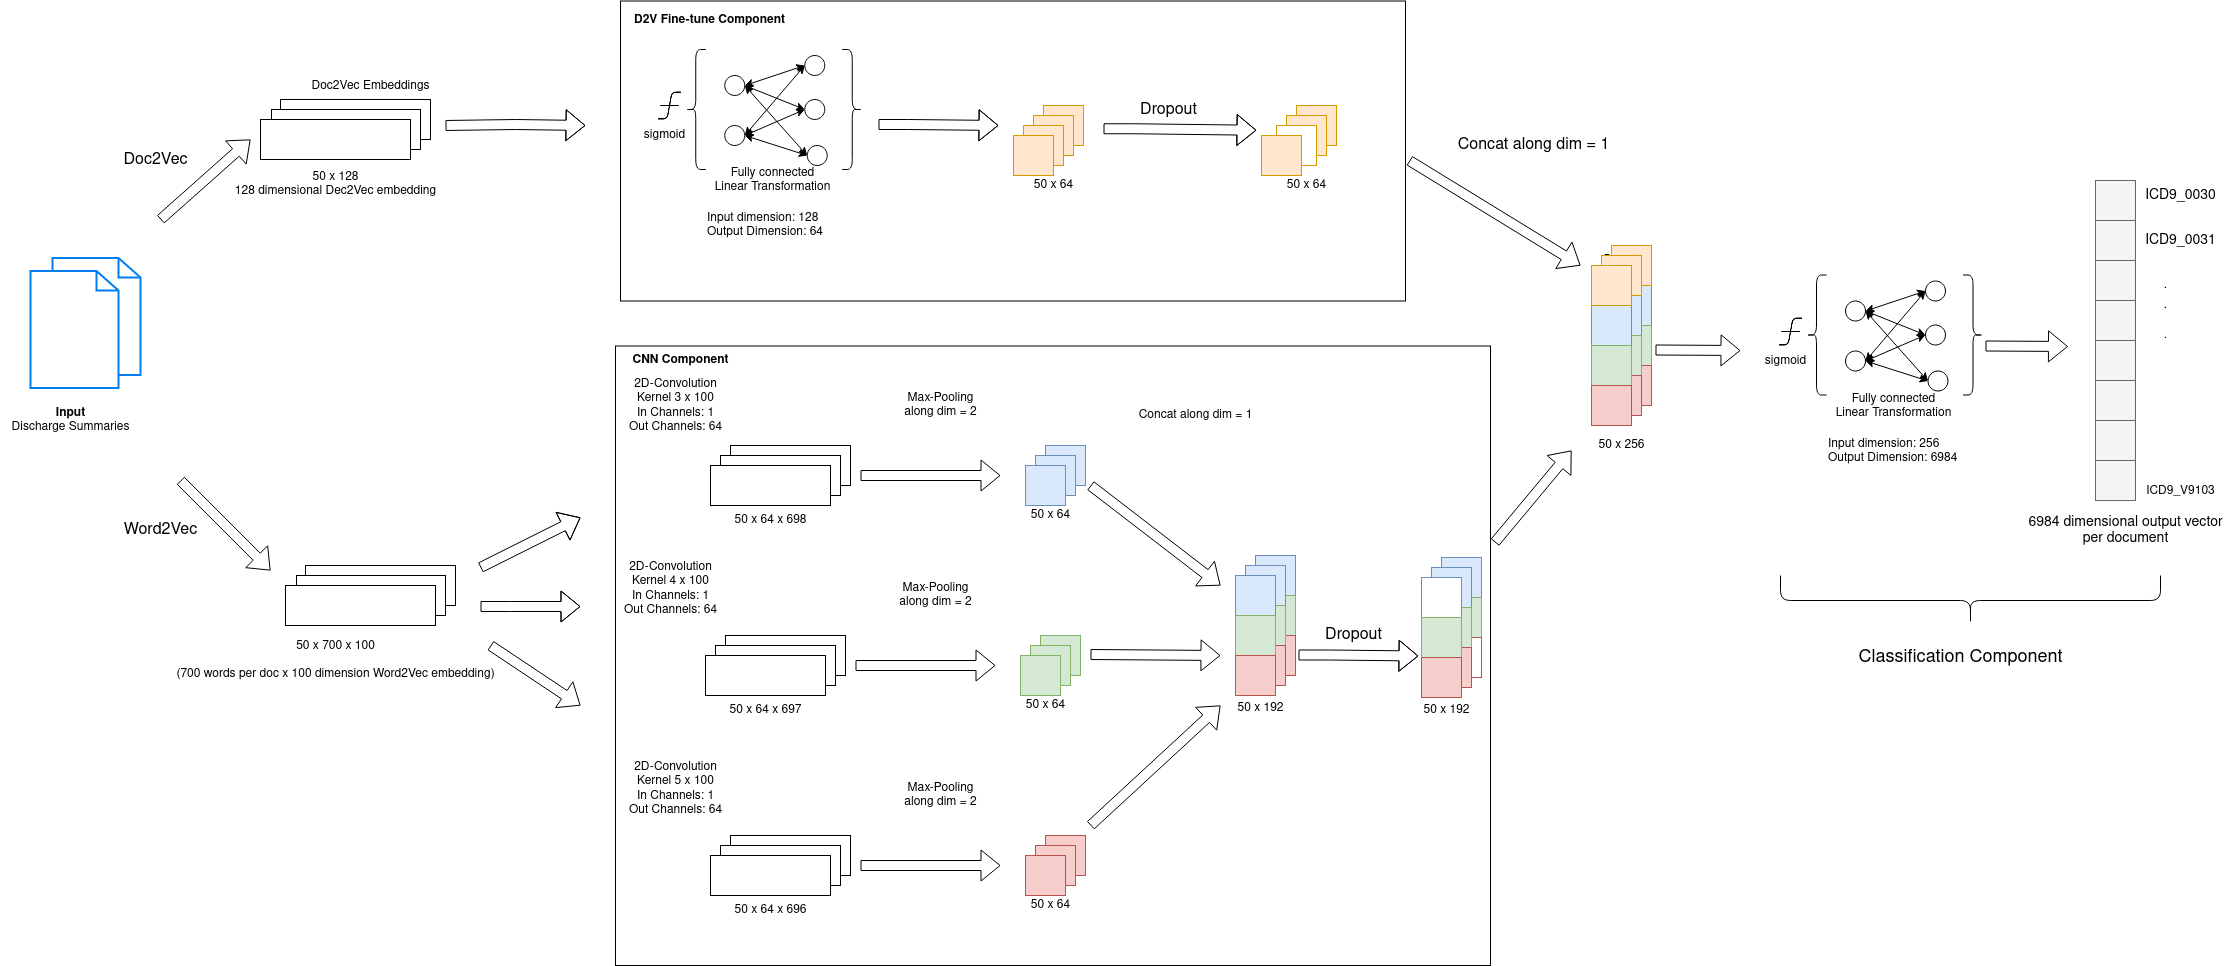
\includegraphics[width=\textwidth,height=4cm]{../src/architecture}
  \caption{Model Architecture}
  \label{arch_diag}
\end{figure*}

The objective is to do end-to-end training of this model. Doc2Vec and Word2Vec models are trained unsupervised, in the pre-processing step. During the supervised learning phase, the above described components are trained for multi-label classification task using back-propagation. The gaol is to achieve similar or close enough performance in terms of micro-averaged F1-score, as achieved in original paper.

The model is medium complexity model in terms of the number of parameters to train.
\newline

\begin{tiny}
\begin{tabular}{ ll }
  \hline
  	CNN layer (300, 400, 500 sized 1D-kernels with 64 channels each) & 76992 \\
  \hline
  	D2V Fine-tune layer (128 input dimension, 64 neurons) & 8256 \\
  \hline
  	Fully-connected classification layer (256 input dimension, 6984 neurons) & 1794888 \\
  \hline
\end{tabular}
\end{tiny}

\subsection{Data descriptions}

The model is trained and tested on MIMIC-III \href{https://physionet.org/content/mimiciii/1.4/}{MIMIC-III} (Medical Information Mart for Intensive Care) database. The data is publicaly available, upon credentiating user identity on Physionet, and completing the mandatory training: Data or Specimens Only Research.

Specifically, following datasets in MIMIC-III were used:

\begin{itemize}
    \item DIAGNOSES\_ICD.csv: Each row in this file maps HADM\_ID (Hospitalization ID) of a patient with a unique ICD9\_CODE. We transform ICD9\_CODE to one-hot encoding and group them per per HADM\_ID to generate multi-hot encoding.
\newline

\begin{small}
\begin{tabular}{ ll }
  \hline
  	Total \# codes & 6984 \\
  \hline
  	Avg. \# codes per patient & 11 \\
  \hline
  	Max \# of codes per patient & 39 \\
  \hline
  	Min \# of codes per patient & 1 \\
  \hline
\end{tabular}
\end{small}

	\item NOTEEVENTS.csv: Each row maps HADM\_ID (Hospitalization ID) with a TEXT (free text Discharge summary) field.
\newline

\begin{small}
\begin{tabular}{ ll }
  \hline
    Total \# discharge summary & 52691 \\
  \hline
    Avg. \# words per discharge summary & 1524 \\ 
  \hline
    Max \# of words per discharge summary & 7980 \\
  \hline
  	Min \# of words per discharge summary & 9 \\
  \hline
\end{tabular}
\end{small}
\end{itemize}


\subsection{Hyperparameters}

TODO

\subsection{Implementation}

The implemenation has been entirely done by the team. To the best of knowledge of the team, no implementation code by authors of original paper, or others is available publicly.

The implementation consists of three Jupyter notebooks:
\begin{itemize}
    \item data-preprocessing.ipynb: This notebook imports the datasets (DIAGNOSES\_ICD.csv and NOTEEVENTS.csv), applies necessary preprocessing and saves the final datasets.
    \item w2v-d2v.ipynb: This notebook generates and saves following:
	\begin{itemize}
		\item \href{https://radimrehurek.com/gensim/models/word2vec.html}{Gensim Word2Vec} model based vectors for all the tokens in the vocabulary of our corpus.
		\item \href{https://radimrehurek.com/gensim/models/doc2vec.html}{Gensim Doc2Vec} model based vectors for all the documents in our corpus.
	\end{itemize}
	\item dl-model.ipynb: This notebook trains and validates the DL model (as described in the model section).
\end{itemize}

Link to source code: \url{https://github.com/manuv3/cs598-dl-project/tree/main/src}


\subsection{Computational requirements}



The computational requirements for different steps are described below:
\begin{itemize}
	\item MIMIC-III datasets import and preprocessing: All the steps were performed on personal machine with 16 GB of total RAM and Intel® Core™ i7-10750H × 12 processor. Only one operation was a bit compute intesive: a "join" operation, during creation of multi-hot ICD9 embeddings for each hospitalization. This operation took around 14 seconds on the CPU of personal machine.
	\item Word2Vec and Doc2Vec model training and vectors generation: All the steps were performed on personal machine. Gensim implementaion of Word2Vec and Doc2Vec support streamed source. So, there is no need to load the whole corpus in memory. However, this is no GPU support in Gensim yet. Since there is no parameter tuning in scope, and this is one time operation, it was performed on personal machine. The time taken to generate these encodings are as folowing:
\newline

\begin{small}
\begin{tabular}{ ll }
	\hline
   		Word2Vec embeddings & 37 minutes \\
  	\hline
    		Doc2Vec embeddings & 51 minutes \\ 
  	\hline
\end{tabular}
\end{small}
\newline
	\item Training the full Deep Learning model: The computational requirements were high due to following factors:
	\begin{itemize}
		\item Each input data to DL model is 70000 dimensional float vector (700 words max with 100 dimensional W2V encoding each). With more than 52600 documents, this requires both large amount of GPU  memory (~14 GB) to store, as well as parallel computing on GPU. Such computing is not possible on available  personal computing environment (correctly predicted in the proposal).
		\item High dimension of problem. There are 6984 ICD9 codes found in the dataset, forming as many dimensions in the multi-label classification problem. As a result the final fully connected layer has over 1.79 million parameters.
	\end{itemize}
	Here, we improve the training time per epoch at the cost of consuming more GPU memory by loading the whole float tensor (52691 x 70000) of size ~14 GB in GPU memory. Such a strategy requires premium GPU  which is available through Google Collab Pro.
	On Colab Pro, we could train and validate the model per run, with following resource utilization:
\newline

\begin{tiny}
\begin{tabular}{ ll }
	\hline
   		System RAM used & 8GB \\
  	\hline
    		GPU RAM used & 23GB (Includes data and model) \\ 
  	\hline
    		Computation units burn rate & 13.08 per hour \\
  	\hline
  		Time taken to train per epoch & 3.5-4 minutes \\
  	\hline
  		Total time taken to run 80 epochs & 5 hours \\
  	\hline
\end{tabular}
\end{tiny}
\newline

Multiple such runs (4 to 5) were executed for hyperparameter tuning.
	\item Training partial model with only D2V (for abalation): During the training of this model we just need to tune the parameters of 2 fully connected layers, which is not very computationally intensive. On Google Collab Free environment, we could achieve this easily:
\newline

\begin{small}
\begin{tabular}{ ll }
	\hline
   		System RAM used & 4.6GB \\
  	\hline
    		GPU RAM used & 1.2GB \\
  	\hline
  		Total time taken to run 80 epochs & 24 minutes \\
  	\hline
\end{tabular}
\end{small}
\newline
	
\end{itemize}


As, estimated during proposal, most of the steps in the whole reproduction process could be performed in personal machine with 16 GB RAM and Intel I7 12-Core CPU. The task of training the main DL model is compute intensive, and required premium GPU support on Google Collab environment.

\section{Results}

The results achieved so far validate the main claim made by the paper, which is that the combined D2V + CNN model performs the multi-label ICD9 classification task with better micro-averaged f1-score, in comparison to traditional ML models: flat-SVM and hierarchical-SVM.

Start with a high-level overview of your results. Does your work support the claims you listed in section 2.1? Keep this section as factual and precise as possible, reserve your judgement and discussion points for the next ``Discussion'' section. 

Go into each individual result you have, say how it relates to one of the claims, and explain what your result is. Logically group related results into sections. Clearly state if you have gone beyond the original paper to run additional experiments and how they relate to the original claims. 

Tips 1: Be specific and use precise language, e.g. ``we reproduced the accuracy to within 1\% of reported value, that upholds the paper's conclusion that it performs much better than baselines.'' Getting exactly the same number is in most cases infeasible, so you'll need to use your judgement call to decide if your results support the original claim of the paper. 

Tips 2: You may want to use tables and figures to demonstrate your results.

% The number of subsections for results should be the same as the number of hypotheses you are trying to verify.

\subsection{Result 1}

We reproduced the DL model, based on D2V and CNN components, to generate document vectors which capture local and global characteristics of the text, and perform multi-lable classification task of identifying the associated ICD9 codes. The result so far are summaried in table below:
\newline

\begin{small}
\begin{tabular}{ ccc }
  \hline
  	Precision & Recall & F1-score \\
  \hline
  	0.467 & 0.344 & 0.396 \\
  \hline
\end{tabular}

\textit{All values are Micro-averaged.}
\end{small}
\newline

The result is based on following hyper-parameters:
\newline

\begin{small}
\begin{tabular}{ ccc }
  \hline
  	Dropout-rate & Probability-Threshold & Epochs \\
  \hline
  	0.20 & 0.20 & 80 \\
  \hline
\end{tabular}

\textit{Probability-Threshold is the threshold for binary classification.}
\end{small}
\newline

\begin{itemize}
	\item The F1-score of 0.396 is better than flat-SVM (0.253) by 36\% and hieerarchical-SVM (0.335) by 15\%.
	\item The F1-score of the model trained so far is 2.9\% worse than the one obtained by authors, in their work.
\end{itemize}

\subsection{Result 2}

We trained a partial DL model (without the CNN component), as part of abalation, to validate the importance of CNN component. The results are provided below:
\newline

\begin{small}
\begin{tabular}{ ccc }
  \hline
  	Precision & Recall & F1-score \\
  \hline
  	0.291 & 0.324 & 0.307 \\
  \hline
\end{tabular}

\textit{All values are Micro-averaged.}
\end{small}
\newline


The f1-score of 0.307 of this partial model is very close to that obtained by original authors 0.308. This result clearly indicates the severe degradation from the performace of combined model, emphasizing the importance of CNN model.

\subsection{Additional results not present in the original paper}

TODO

\section{Discussion}

The original paper is reproducible to a large extent. Based on the results achieved so far, perfomance claim on the main model has been reached within 3\% of original values. Moreover, it has been conclusively proved that the proposed model improves on the performance of baseline models by 15-36\%.

The results also validates the overall approach taken:
\begin{itemize}
	\item Maintain the quality and quantity of data, to ensure that some important features are not missed due to any data loss.
	\item Do not alter the main parameters of the model (as proposed by authors) like word/document embedding lengths, kernel sizes, count of activation units, number of layers, etc.
	\item Vary the hyperparameters like dropout rate, classification threshold etc. to achieve the desired performance metrics. 
\end{itemize}

One weakness of the approach was to not plan for faster and cheaper way to perform hyper-parameter tuning (like using a smaller subset of data to get quick feedback). So long training duration (of about 5 hrs for 80 epochs) was costly, as well as limited the ability of experiment with hyper-parameters.

As next steps, we want to:
\begin{itemize}
	\item do more hyper-parameter tuning and possibly run more number of epochs, in the effort to bring the model performance closer original authors' model.
	\item train another model without D2V component to ascertain the its importance, as part of abalation.
	\item try changing the base parameters like number of kernel size in CNN component, or number of neurons in D2V component, etc., and observing the impact on model performance.
\end{itemize}




\subsection{What was easy}
\begin{itemize}
	\item It is relatively easy to obtain the raw MIMIC-III data, and be able to extract almost same amount of samples as used by original authors, with basic pre-processing. 
	\item It was easy to train Gensim Word2Vec and Doc2vec models. Gensim library is pretty stable, and intuitive to use, with decent documentation.
\end{itemize}

\subsection{What was difficult}
\begin{itemize}
	\item The authors left some gaps in describing the architecture of the model. For example, the architecture of D2V fine-tuning layer was not clarified. The overall architecture diagram provided by authors is abstract and leaves out finer details like which activation functions were used in DL layers. So, it was an effort to bridge some missing pieces.
	\item The size of the model is relatively big, and lots of time was spent during training cycles. Also, cloud computing costs added up, due to intensive use of GPU.
\end{itemize}

\subsection{Recommendations for reproducibility}
\begin{itemize}
	\item The authors should provide more detailed architecture of the DL model. For example, where exactly are the dropout layers located in the model, what are the actual activation functions used, etc.
	\item The authors should give more detailed description of the implementation. For example, what was their training environment, what data pre processing steps did they perform, how many epochs did they run, etc.
\end{itemize}


\section{Communication with original authors}

No communication happened with original authors, so far.


\bibliographystyle{plain}
\bibliography{acl2021}

%\appendix



\end{document}

